\documentclass{sigchi}

% Load basic packages
\pagenumbering{arabic}
\usepackage[utf8]{inputenc}
\usepackage[ngerman]{babel}
\usepackage{balance}  % to better equalize the last page
\usepackage{graphics} % for EPS, load graphicx instead 
%\usepackage[T1]{fontenc}
\usepackage{txfonts}
\usepackage{times}    % comment if you want LaTeX's default font
\usepackage[pdftex]{hyperref}
% \usepackage{url}      % llt: nicely formatted URLs
\usepackage{color}
\usepackage{textcomp}
\usepackage{booktabs}
\usepackage{ccicons}
\usepackage{todonotes}

% llt: Define a global style for URLs, rather that the default one
\makeatletter
\def\url@leostyle{%
  \@ifundefined{selectfont}{\def\UrlFont{\sf}}{\def\UrlFont{\small\bf\ttfamily}}}
\makeatother
\urlstyle{leo}

% To make various LaTeX processors do the right thing with page size.
\def\pprw{8.5in}
\def\pprh{11in}
\special{papersize=\pprw,\pprh}
\setlength{\paperwidth}{\pprw}
\setlength{\paperheight}{\pprh}
\setlength{\pdfpagewidth}{\pprw}
\setlength{\pdfpageheight}{\pprh}

% Make sure hyperref comes last of your loaded packages, to give it a
% fighting chance of not being over-written, since its job is to
% redefine many LaTeX commands.
\definecolor{linkColor}{RGB}{6,125,233}
\hypersetup{%
  pdftitle={SIGCHI Conference Proceedings Format},
  pdfauthor={LaTeX},
  pdfkeywords={SIGCHI, proceedings, archival format},
  bookmarksnumbered,
  pdfstartview={FitH},
  colorlinks,
  citecolor=black,
  filecolor=black,
  linkcolor=black,
  urlcolor=linkColor,
  breaklinks=true,
}

\begin{document}

\title{Energieeffizienz durch Computation Offloading in der Cloud}

\numberofauthors{1}
\author{
  \alignauthor{Matthias Fey\\
    \affaddr{TU Dortmund, Fakultät für Informatik}\\
    \affaddr{Otto-Hahn-Straße 14}\\
	\affaddr{44227 Dortmund, Germany}\\
    \email{matthias.fey@tu-dortmund.de}}\\
}

\maketitle

\begin{abstract}

Die Popularität von Smartphones und dessen Applikationen ist innerhalb der letzten Jahre stark gestiegen.
Aber so sehr der App-Markt explodiert und immer komplexer werdende Programme wie Objekterkennung oder Videobearbeitung auf Smartphones zur Verfügung stehen, so unglücklicher werden Benutzer mit der Akkulaufzeit dieser.
Energieeffizienz ist daher ein wichtiges Thema bei der Entwicklung von benutzerfreundlichen mobilen Applikationen.
Computation Offloading, d.h. die Auslagerung von komplexen Berechnungen an leistungsstärkere Computer, ist ein möglicher Anwärter für die Erstellung energieeffizienterer Applikationen.

Diese Arbeit beleuchtet das Computation Offloading und zeigt den aktuellen Stand dessen in der Forschung auf.
Neben der Grundidee des Computation Offloadings und der Vorstellung bisheriger Arbeiten auf diesem Gebiet, beschäftigt sich diese Arbeit vor allem mit der Frage, ob Computation Offloading eine geeignete Möglichkeit darstellt, energieeffizientere Applikationen zu entwickeln.
\end{abstract}

\section{Einleitung}

Das Smartphone revolutioniert unser Leben.
So warb Apple schon 2010 mit dem Slogan \glqq There's an app for everything\grqq\ und zeigt damit auf, wohin die Reise geht.
Mittlerweile surfen wir im Internet, checken unsere Emails, gucken Videos und betreiben Social Media auf unseren mobilen Endgeräten.
Dabei können wir dank zusätzlichen Komponenten und Sensoren am Smartphone wie Kamera oder GPS sogar weitaus mehr bewerkstelligen als am Computer und sind dabei noch mobil.
Das App-Geschäft explodiert.
So finden täglich neue innovative und revolutionäre Applikationen ihren Weg in die gegenwärtigen Smartphone Stores.
Laut Forschung wächst die App-Industrie im Jahr 2015 exponentiell auf einen Marktwert von 37 Milliarden an~\$ \cite{e3-1}.

Das Smartphone ist ebenso alltäglich geworden. Haben wir es nicht bei uns oder neigt sich der Akku dem Ende fühlen wir uns unverzüglich eingeschränkt in unseren Fähigkeiten.
Das hat zur Folge, dass wir bei geringer Akkulaufzeit unseren Konsum ungewollt drosseln und unser Smartphone daher nicht zu vollem Potenzial nutzen können.
Je mehr unsere Nachfrage nach komplexer werdenden Programmen auf Smartphones steigt, umso unglücklicher werden wir mit der Akkulaufzeit dieser.
Eine Umfrage mit tausenden von Smartphone-Nutzern hat ergeben, dass die Verbesserung der Akkulaufzeit der größte Wunsch des Endnutzers ist~\cite{o13-6}.

Der Nutzen eines Smartphones ist und bleibt limitiert durch dessen Akkulaufzeit.
Die Batteriekapazität wird dabei gravierend eingeschränkt durch die Größe und das Gewicht der Endgeräte.
Das hat zur Folge, dass die Energiedichte von Batterien in Smartphones mit einer recht unbedeutenden Rate von nur 5\% jährlich anwächst~\cite{o12-8}. 
Größere Smartphones mit stärkeren Akkus sind jedoch keine attraktive Alternative.
Ebenso schmälern thermische Anforderungen die Leistung von Smartphones auf ungefähr 3 Watt~\cite{o12-5}.

Energieeffizienz ist daher ein wichtiges aber ebenso auch unterschätztes Thema bei der Entwicklung von benutzerfreundlichen mobilen Applikationen.
Optimales Energiemanagement erfordert ein gutes Verständnis über die Energienutzung von Smartphones~\cite{e1}.
Es ist folglich nicht verwerflich, dass Entwickler sich bisher nur wenige Gedanken um Energieeffizienz in ihren Applikationen gemacht haben~\cite{e3}.
So verbrauchen 6 der 10 beliebtesten Apps im Google Play Store über einer Laufzeit von 30 Sekunden bis zu 0,75\% einer vollen Akkuladung~\cite{e3}.

In dieser Arbeit wird das \emph{Computation Offloading in der Cloud} als Möglichkeit zur Energieeinsparung in Smartphone-Applikationen vorgestellt.
Computation Offloading bedeutet, dass komplexe Aufgaben oder Berechnungen in mobilen Applikationen an leistungsstärkere Computer (zum Beispiel die Cloud) ausgelagert werden.
Im nachfolgenden Kapitel wird auf die Grundidee des Offloadings und insbesondere auf dessen Entscheidungsfindung eingegangen:
Wann ist Offloading überhaupt praktikabel?
Wie werden mögliche Bereiche einer Applikation für das Offloading bestimmt?
Und welche Typen von Applikationen können beispielsweise durch Computation Offloading energieeffizienter gestaltet werden?

Daraufhin werden bisherige Arbeiten in diesem Forschungsgebiet vorgestellt.
Es wurden in der Vergangenheit bereits eine Vielzahl von Frameworks entwickelt, die CPU intensive Aufgaben automatisiert auslagern~\cite{thinkair, maui, clonecloud, cuckoo, moca, smartdiet}.
Mit besonderem Augenmerk wird hier das Framework ThinkAir~\cite{thinkair} präsentiert, welches sich die Frameworks MAUI~\cite{maui} und CloneCloud~\cite{clonecloud} zu Nutzen macht.

Im nachfolgenden Abschnitt werden Ergebnisse aus verschiedenen Studien mit unterschiedlichen Testszenarien und Übertragungstechnologien präsentiert~\cite{o2, o8, o12, thinkair}.
In einer anschließenden Diskussion wird kritisch auf die Frage eingegangen, ob sich Offloading im alltäglichen Gebrauch lohnt und wo mögliche Schwächen liegen.
Zum Abschluss wird ein Ausblick auf die Zukunft des Computation Offloadings gegeben.

\section{Computation Offloading}

Computation Offloading (oder \emph{cyber foraging} bzw. \emph{surrogate computing} \cite{o4}) ist die englische Bezeichnung für die Auslagerung von komplexen Aufgaben oder Berechnungen an leistungsstärkere Computer (zum Beispiel die Cloud) über Netzwerkübertragung.
Dafür werden die entsprechenden Daten für die Berechnung vom Smartphone an den entsprechenden Offloading-Server gesendet.
Das Smartphone wartet auf die Abarbeitung der Berechnung und empfängt nach Fertigstellung die berechneten Ergebnisse vom Server.
Durch die Auslagerung verspricht man sich zum einen den Gewinn an Performance (d.h. die schnellere Abarbeitung der Aufgabe und die Nutzung der freigewordenen Ressourcen für andere Funktionen) und zum anderen die Einsparung von Energiekosten auf dem Smartphone.

\begin{figure}
\centering
  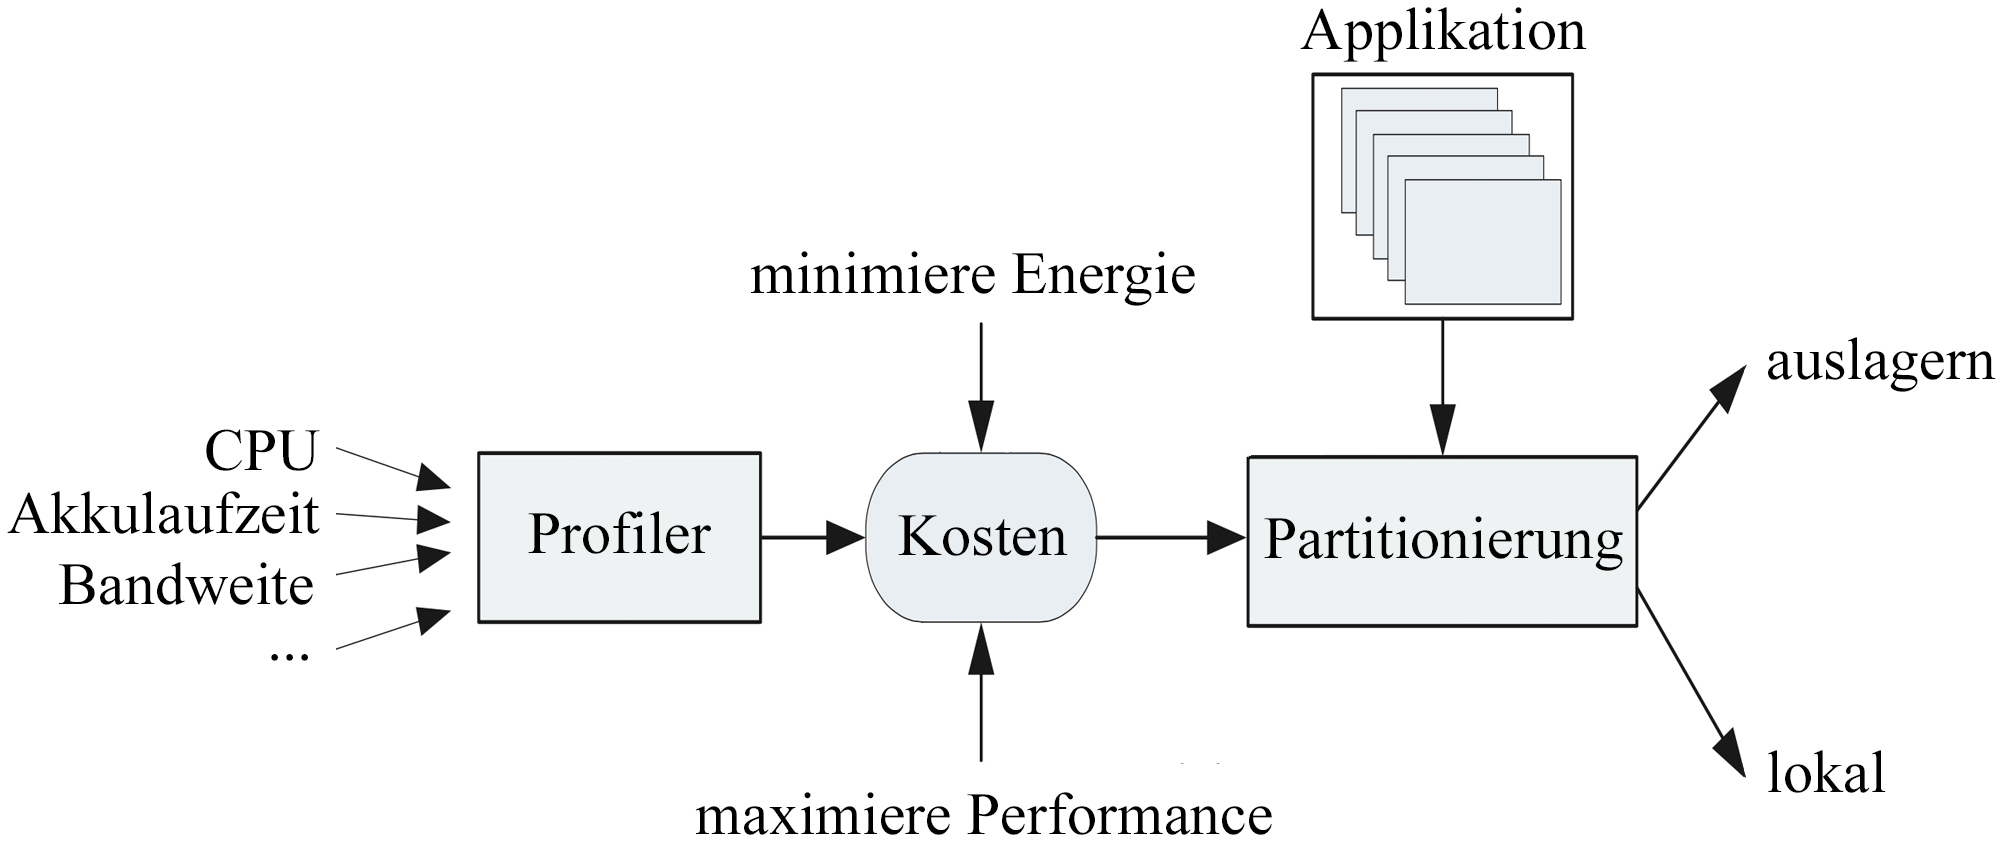
\includegraphics[width=1.0\columnwidth]{images/architektur}
  \caption{Architektur von Computation Offloading Systemen nach~\protect\cite{O13}}\label{fig:architektur}
\end{figure}

Die typische Architektur von Computation Offloading Systemen bestehend aus drei Hauptkomponenten (Profiler, Kostenmodell und Partitionierung) zeigt Abbildung~\ref{fig:architektur}.

\emph{Profiler} sammeln wertvolle Informationen wie CPU-Auslastung, Akkulaufzeit und Bandbreite über das Smartphone und dessen Netzwerkumgebung~\cite{O13}.
Sie sollen dabei möglichst genaue Angaben liefern und dabei so wenig Leistung wie möglich in Anspruch nehmen, um den zusätzlichen Mehraufwand der Applikation für das Computation Offloading gering zu halten~\cite{thinkair}.

Die Schlüsselkomponente der Architektur ist das \emph{Kostenmodell}.
Hier wird anhand von Kriterien und den Profiler-Informationen die Entscheidung getroffen, wann und welche Komponenten bzw. Methoden einer Applikation in die Cloud ausgelagert werden sollen.
In der Abbildung werden die Kriterien \glqq minimiere Energie\grqq\ und \glqq maximiere Leistung\grqq\ genannt.
Es sind aber ebenso auch andere Kriterien denkbar wie das Maximieren von Sicherheit und Datenschutz oder Robustheit der Applikation~\cite{O13}.
Diese Arbeit beschäftigt sich im weiteren Verlauf aber nur mit der Einsparung von Energie als Kriterium.

Die \emph{Partitionierung} teilt die Applikation anhand der Ergebnisse des Kostenmodells in zwei Bereiche: eine lokale Partition, die auf dem mobilen Endgerät ausgeführt wird und eine Partition, die in die Cloud ausgelagert wird~\cite{O13}.

Die Cloud bietet dabei den idealen Platz für die Auslagerung von komplexen Berechnungen dank ihrer einfachen Skalierbarkeit.
Sie bietet nahezu unendlich viele Ressourcen, die auf Nachfrage und je nach Auslastung zur Verfügung stehen~\cite{o12}.
Ebenso bietet sie den Vorteil des Multitaskings und kann damit mehrere Applikationen und Prozesse simultan laufen lassen~\cite{o4}.
Die Popularität der Cloud liegt unter anderem auch daran, dass sie relativ kostengünstig ist~\cite{O13}.

\subsection{Trade-off}

Es ist wichtig anzumerken, dass Computation Offloading eine opportunistische Möglichkeit zur Erstellung von energieeffizienten Applikationen ist, aber keinesfalls eine Pflicht für zukünftige Programme darstellt.
Das liegt insbesondere an den zusätzlichen Energie- und Netzwerkkosten für die Datenübermittlung, die natürlich bei der Entscheidung für die Auslagerung bedacht werden müssen.~\cite{O13, o2}.
Die Abwägung (engl. \emph{Trade-off}~\cite{o8}) zwischen dem Energieverbrauch zur Auslagerung der Aufgabe und der Energieeinsparung dank der Cloud entscheidet darüber, wann und ob Computation Offloading überhaupt sinnvoll ist.
Dieser Trade-off lässt sich mathematisch wie folgt definieren~\cite{o8}: 

\begin{equation*}
	E_{\textit{trade}} = E_{\textit{lokal}} -E_{\textit{offload}} > 0
\end{equation*}

$E_{\textit{lokal}}$ bezeichnet dabei die Energie, die durch lokale Berechnung auf dem Smartphone verbraucht wird und $E_{\textit{offload}}$ kennzeichnet den Energieverbrauch durch die Auslagerung der Aufgabe auf der Seite des Smartphones.
Nur wenn $E_{\textit{trade}}$ positiv ist, wird mit Hilfe von Computation Offloading Energie auf dem Smartphone eingespart.

Da sich Energie über die durchschnittliche Leistung über einen bestimmten Zeitraum bestimmt ($E = P \times T$), lässt sich $E_{\textit{lokal}}$ weiter auflösen.
Sei $C$ dafür die Komplexität der Aufgabe (Anzahl auszuführender Anweisungen), $X_{\textit{lokal}}$ die Geschwindigkeit der lokalen Berechnung und $P_{\textit{lokal}}$ die benötigte Leistung zur lokalen Berechnung, dann gilt~\cite{o8}:

\begin{equation*}
	E_{\textit{lokal}} = \frac{P_\textit{lokal} \times C}{X_\textit{lokal}}
\end{equation*}

Die Energiekosten zur Auslagerung der Aufgabe $E_{\textit{offload}}$ setzen sich dagegen aus den Kosten zum Senden der Daten an die Cloud $E_{\textit{senden}}$, zum Warten auf die Beendigung der Berechnung in der Cloud $E_{\textit{warten}}$ und zum Empfangen des Ergebnisses $E_{\textit{empfangen}}$ zusammen~\cite{o8}:

\begin{equation*}
	E_{\textit{offload}} = E_{\textit{senden}} + E_{\textit{warten}} + E_{\textit{empfangen}}
\end{equation*}

Diese Energien lassen sich erneut mit Hilfe der Beziehung zwischen Leistung und Zeit zum Energieverbrauch auflösen~\cite{o8}:

\begin{equation*}
	E_{\textit{offload}} = P_s \times T_s + P_w \times T_w + P_e \times T_e
\end{equation*}

\begin{figure}
\centering
  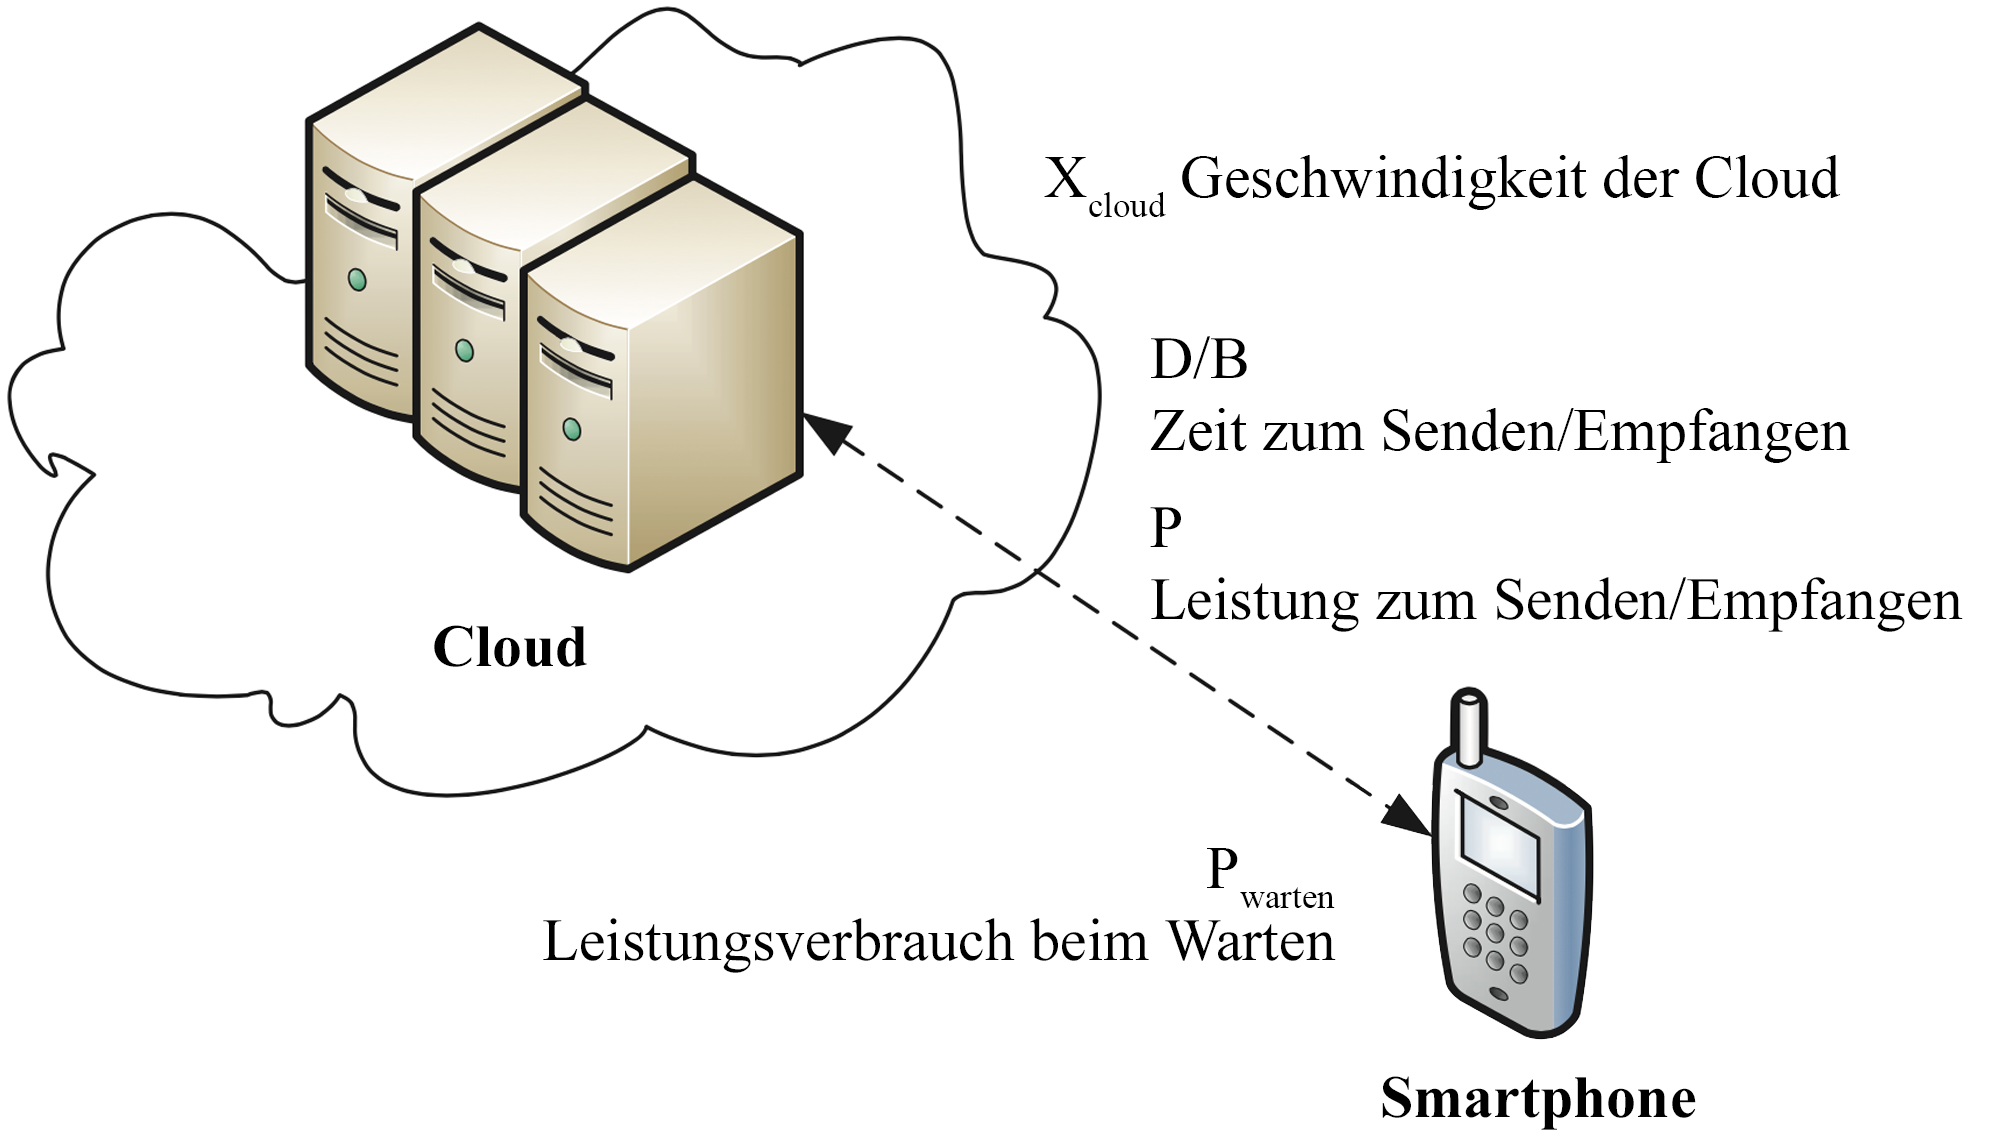
\includegraphics[width=1.0\columnwidth]{images/trade-off}
  \caption{Energiekosten eines Offloading-Prozesses nach~\protect\cite{O13}}\label{fig:trade-off}
\end{figure}

Abbildung~\ref{fig:trade-off} veranschaulicht den Energieverbrauch bei der Auslagerung der Berechnung und die davon abhängigen Variablen.

Die Zeit des Wartens $T_w$ ist von der Aus\-füh\-rungs\-ge\-schwin\-dig\-keit der Cloud $X_{\textit{cloud}}$ abhängig.
Ebenso lassen sich die Zeitintervalle zum Senden $T_s$ und Empfangen $T_e$ der Daten über die Menge der zu verschickenden und zu empfangenden Daten $D_s$, $D_e$ sowie die aktuellen Bandbreiten $B_s$, $B_e$ berechnen~\cite{o8}.
Die Netzwerklatenzen seien hier mit in der Bandbreite berücksichtigt.
Es ergibt sich damit:

\begin{align*}
	& & E_{\textit{trade}} = & \,\frac{P_{\textit{lokal}} \times C}{X_\textit{lokal}} - \frac{P_w \times C}{X_{\textit{cloud}}} - \frac{P_s \times D_s}{B_s} - \frac{P_e \times D_e}{B_e} & > 0 \\
	& \Leftrightarrow & E_{\textit{trade}} = & \, C\left( \frac{P_{\textit{lokal}}}{X_\textit{lokal}} - \frac{P_w}{X_{\textit{cloud}}} \right) - P_s\frac{D_s}{B_s} - P_e\frac{D_e}{B_e} & > 0 \\
\end{align*}

$P_{\textit{lokal}}/X_{\textit{lokal}} - P_{\textit{w}}/X_{\textit{cloud}}$, $P_s$ und $P_w$ sind geräteabhängige, unveränderliche Werte des jeweiligen Smartphones und der jeweiligen Cloud-Plattform.
Es wird damit ersichtlich, dass eine hohe Komplexität der auszulagernden Aufgabe das Computation Offloading befürwortet, wohingegen eine geringe Bandbreite oder ein hoher Datenaustausch zwischen den Geräten die Vorteile von Offloading mildern~\cite{o8}.

\subsection{Statisch vs. dynamisch}

Die Wahlmöglichkeit, welche Bereiche einer Applikationen geeignete Kandidaten für die Auslagerung darstellen, kann entweder statisch oder dynamisch von Statten gehen.
Bei der statischen Entscheidung wird die Applikation bereits während der Entwicklung in die jeweiligen lokalen und auszulagernden Bereiche partitioniert~\cite{o4}.
Die Applikation wird direkt als Computation Offloading System geplant und kann deshalb im späteren Verlauf nur schwer rückgängig gemacht werden.
Das hat wiederum den Vorteil, dass kein Mehraufwand der Applikation für Profiler während der Laufzeit bewerkstelligt werden muss~\cite{o4}.
Im Vorfeld müssen jedoch die Parameter, die die Trade-off-Ungleichung bestimmen, möglichst präzise prognostiziert werden.
Die Parameter $C$, $P_{\textit{lokal}}$, $P_w$, $X_{\textit{lokal}}$, $P_s$, $P_e$ und $D_e$ können üblicherweise vorausschauend kalkuliert werden.
 Die Geschwindigkeit der Cloud $X_{\textit{cloud}}$ kann variieren, jedoch garantieren die meisten Cloud-Anbieter ein Minimum an Performance~\cite{o4}.
 Die Bandbreiten $B_s$ und $B_e$ können nur schwer während der Entwicklung geschätzt werden.
 Ebenso können die zu versendenden Daten $D_s$ stark von der jeweiligen Anforderung abhängen.
 Ein statisches Computation Offloading System kann aber mittels Wahrscheinlichkeitsrechnung oder Fuzzy-Regelungen versuchen, auch diese Parameter vorherzusagen~\cite{o4}.

Im Gegensatz dazu kann ein dynamisches Computation Offloading System auf verschiedene Umgebungsbeschaffenheiten während der Laufzeit reagieren, zum Beispiel bei schwankenden Netzwerkbandbreiten~\cite{o4}.
Ein Profiler und ein Kostenmodell entscheiden dann während der Ausführung der Applikation darüber, ob es sich lohnt eine Berechnung auszulagern (vgl. Abbildung~\ref{fig:architektur}).
Das hat den Nachteil, dass die Parameter zur Entscheidungsfindung über den gesamten Zeitraum der Applikation überwacht werden müssen.
Die Überwachung dieser Parameter ist aber mittlerweile relativ kostengünstig, so dass sich der Mehraufwand dafür in Grenzen hält~\cite{thinkair}.
Auf der anderen Seite sind der Profiler und das Kostenmodell auch im späteren Verlauf der Entwicklung oder nach der Veröffentlichung leicht erweiterbar bzw. anpassbar, um auch auf zukünftige Ansprüche schnell zu reagieren.
Welche Bereiche einer Applikation potenziell ausgelagert werden wird auch in einem dynamischen System meistens statisch identifiziert.
Eine Partitionierung während der Laufzeit stellt einen zu hohen, unerwünschten Mehraufwand für die Analysierung des Programms dar~\cite{o4}.
Forschungsarbeiten, die sich mit Computation Offloading Systemen beschäftigen, erlebten im Laufe der Jahre einen Umbruch von statischen hinzu dynamischen Systemen~\cite{o4}.
Das liegt unteranderem auch daran, dass dynamische Systeme weitaus automatisierter arbeiten und dem Entwickler damit eine Menge Arbeit abnehmen.

\subsection{Applikationen}

Es gibt eine unzählige Anzahl von Applikationen, die in verschiedener Art und Weise für Computation Offloading in Frage kommen.
Generell ziehen Applikationen mit komplexen Methoden und wenig Datenaustausch den größten Nutzen aus der Auslagerung.
Als Beispiel dafür sind zum Beispiel Texteditoren zu nennen, die eine geringe Menge von Daten $D_s$ verschicken und darauf beispielsweise eine Rechtschreibüberprüfung in der Cloud durchführen~\cite{o4}.
Als weiteres Beispiel für wenig Datenaustausch sei hier eine Schach-KI zu nennen mit der Einschränkung, dass die Entscheidung zur Auslagerung zusätzlich von der Fähigkeit des Spielers abhängig ist.
Um einen guten Spieler zu schlagen, muss die Künstlich Intelligenz eine Mehrzahl an Berechnungen durchführen und folglich wird Computation Offloading  gegen erfahrene Spieler profitabler~\cite{o4}. 

Applikationen wie Videobearbeitung oder Objekterkennung transferieren große Datenmengen zur Cloud und die Einsparung von Energie hängt damit größtenteils von der Bandweite $B_s$ ab.
Bezieht man sich auf Videos oder Bilder im Internet (zum Beispiel YouTube), so ist Computation Offloading natürlich profitabler~\cite{o4}.

Weitere Typen von Applikationen sind zum Beispiel Sprach\-er\-kenn\-ungs-~\cite{thinkair}, Augmented Reality-~\cite{O13} oder Da\-ten\-analyse-Programme für Gesundheit und Fitness~\cite{clonecloud} sowie Virusscanner~\cite{thinkair}.

\section{Bisherige Arbeiten}

Der Energieverbrauch einer Applikation hängt stark davon ab, auf welchem System und auf welcher Hardware diese ausgeführt wird~\cite{seeds}.
Eine vor kurzem erfolgte Studie zeigt auf, dass mehr als 10.000 mögliche Kombinationen bezüglich Hardware und Software für Android-Applikationen existieren~\cite{seeds-34}.
Es gibt natürlich Kombinationen, die allgemein üblicher sind als andere, aber für Entwickler sind es dennoch zu viele, um diese zu berücksichtigen~\cite{seeds}.
Es bietet sich demnach an, Systeme bzw. Frameworks zu benutzen, die einem diesen Entscheidungsprozess abnehmen.

Es wurden über die Jahre eine Menge von Frameworks (hauptsächlich für Android-Systeme) vorgestellt, die dem Entwickler bei der Aufgabe des Computation Offloadings helfen~\cite{o4}.
Neuere Systeme sind zum Beispiel \emph{ThinkAir}~\cite{thinkair}, \emph{MAUI}~\cite{maui}, \emph{CloneCloud}~\cite{clonecloud}, \emph{Cuckoo}~\cite{cuckoo}, \emph{MOCA}~\cite{moca} und \emph{SmartDiet}~\cite{smartdiet}.
Diese bieten unterschiedliche Ansätze und Lösungen zur Verbesserung des Computation Offloadings und adressieren unter anderem auch Thematiken wie Transparenz und Sicherheit für den Benutzer~\cite{o4}.

MAUI unterstützt beispielsweise wie viele andere existierende Frameworks die Partitionierung der Applikationen über die Annotierung von Methoden~\cite{maui}.
Methoden, die potenziell ausgelagert werden sollen, werden somit als solche gekennzeichnet.
Allerdings berücksichtigt MAUI nicht die Möglichkeit zur Skalierierbarkeit der Cloud und verschenkt damit Potenzial~\cite{maui, thinkair}.

CloneCloud migriert einen laufenden Thread im Smartphone zu einem bestimmten Zeitpunkt zu einem Applikationsklon in der Cloud~\cite{clonecloud}.
Es bestimmt diesen Zeitpunkt mit Hilfe einer statischen Analyse.
Die Threads werden auf dem Smartphone und in der Cloud unter verschiedenen Laufzeitbedingungen ausgeführt und analysiert~\cite{clonecloud}.
CloneCloud bestimmt damit, welche Threads zu welchem Zeitpunkt und unter welchen Bedingungen in die Cloud ausgelagert werden sollen.
Damit limitiert sich dieser Ansatz durch die statische Analyse und berücksichtigt keine Veränderungen der Umgebung während der Laufzeit.~\cite{thinkair}.
Außerdem muss die statische Analyse für jede neue Applikationsversion neu ausgeführt werden~\cite{thinkair}.

ThinkAir bedient sich aus dem Besten der beiden oben genannten Frameworks~\cite{thinkair}.
Dabei adressiert es die fehlende Skalierbarkeit von MAUI, in dem es je nach Auslastung dynamisch eine parallel laufende Anzahl von virtuellen Maschinen eines Smartphone-Klons in der Cloud erstellt oder zerstört~\cite{thinkair}.
Im Gegensatz zu CloneCloud bietet ThinkAir die Auslagerung von Methoden anstatt von Threads und einen Profiler, der während der Ausführung Informationen zur Entscheidungsfindung liefert~\cite{thinkair}.
ThinkAir ist damit ein dynamisches System und kann folglich schnell auf Veränderungen der Umgebung reagieren um stets die richtige Entscheidung zu treffen.
Mittels eines einfachen Interfaces ist es für Entwickler einfach zu benutzen und mindert die Gefahr, dass Framework sinnwidrig zu benutzen.
Im folgenden Verlauf des Kapitels soll das ThinkAir-Framework nach~\cite{thinkair} näher erläutert werden. 

ThinkAir besteht aus drei wesentlichen Komponenten: Der Smartphone-Umgebung, dem Applikationsserver und den Profilern.

\subsubsection{Smartphone-Umgebung}

ThinkAir bietet eine einfach zu benutzende Bibliothek für die potenzielle Auslagerung von Methoden für Android-Applikationen.
Jede Methode, die es wert sein könnte, ausgelagert zu werden, wird vom Entwickler als solche mit \texttt{@Remote} annotiert.
Der Aufruf dieser Methode erfolgt dann automatisch im \texttt{ExecutionController}, der mittels verschiedener Kriterien darüber entscheidet, ob die Methode lokal oder in der Cloud ausgeführt werden soll.
Die Entscheidung ist dabei abhängig von den gesammelten Umgebungsdaten der Profiler sowie von vergangenen Entscheidungen und Informationen zur Ausführung dieser Methode.
Gibt es noch keinen vorangegangen Aufruf dieser Methode, basiert die Entscheidung des \texttt{ExecutionControllers} nur auf den Umgebungsparametern der Profiler.
Gibt es beispielsweise eine signalstarke WiFi-Verbindung, so wird die Methode aller Voraussicht nach ausgelagert.
Auf einer signalschwachen Verbindung wird die Methode eher lokal ausgeführt.
Beim Aufruf sammeln die Profiler dann Daten über Ausführungszeit und Energieverbrauch und trainieren damit den \texttt{ExecutionController} auf bessere Entscheidungsfindung.
Wird eine Methode ausgelagert und die Verbindung schlägt aus unbekannten Gründen fehl, wird die Methode lokal ausgeführt.
Damit ist sichergestellt, dass die Benutzung der Applikation auch bei Verbindungsabbrüchen weiter funktioniert.

\subsubsection{Applikationsserver}

Der Applikationsserver kümmert sich auf Seiten der Cloud um den auszulagernden Quelltext und dessen Ausführung.
Ein \texttt{ClientHandler} registriert jede neue Client-Verbindung sobald sich ein neuer ThinkAir-\texttt{ExecutionController} mit der Cloud verbindet.
Ist die Applikationssoftware der Cloud unbekannt, lädt der \texttt{ClientHandler} den Quelltext vom Smartphone und kümmert sich automatisch um die Einbindung aller nötigen nativen Bibliotheken.
Ebenso antwortet der \texttt{ClientHandler} auf alle Ping-Nachrichten für die Bestimmung der aktiven Verbindungslatenz.

Wirft der Applikationsserver beim Berechnen eine \texttt{OutOfMemory}-Exception, wird die Methode nicht lokal auf dem Smartphone neugestartet.
Stattdessen kümmert sich der Applikationsserver selbstständig um die Umschichtung der Aufgabe auf eine andere leistungsstärkere virtuelle Maschine.
Ebenso kann der Client explizit nach mehr Leistung fragen.

Der Applikationsserver nutzt eine Virtualisierungsplattform und kann damit auf privaten sowie kommerziellen Clouds zum Einsatz kommen.
Als Plattformen sind zum Beispiel Xen, QEMU und VirtualBox von Oracle zu nennen.
Virtualisierung auf der Cloud hat gegenüber Smartphones den enormen Vorteil, dass Multitasking weitaus effizienter über Multiprozessoren oder über die Erweiterung zu mehreren virtuellen Maschinen ausgenutzt werden kann.

\subsubsection{Profiler}

Das Profiler-System ist hochgradig modular um die Einbindung von neuen Profilern leicht zu ermöglichen.
Aktuell besitzt ThinkAir vier Profiler (Hardware, Software, Netzwerk, Energie), die sich um das Sammeln von verschiedenen Daten kümmern.
Insbesondere werden \texttt{Listener} mit dem System registriert, um eine Übersicht über die Akkulaufzeit, die Verbindungsstärke und dessen Technologie (Wifi, 3G, ...) zu erhalten.
Dadurch werden keine zusätzlichen Ressourcen für die Ermittlung dieser Daten benötigt.
Die vier Profiler ermitteln unter anderem folgenden Daten:
\begin{itemize}
	\item \textbf{Hardware:} CPU-Auslastung, Display-Helligkeit, Verbindung, ...
	\item \textbf{Software:} Ausführungszeit und Komplexität von Methoden, Anzahl von Methodenaufrufen, ... (Ermittlung über Android Debug API)
	\item \textbf{Netzwerk:} Round Trip Time (RTT) und Datenrate (Abschätzung der vorliegenden Bandbreite), Anzahl gesendeter und empfangener Pakete pro Sekunde, ...
	\item \textbf{Energie:} Geschätzter Energieverbrauch von Methodenaufrufen
\end{itemize}

Um den Energieverbrauch einzelner Methoden dynamisch zur Laufzeit zu ermitteln, macht sich ThinkAir das \emph{PowerTutor}-Modell zu Nutze~\cite{powertutor}.
PowerTutor ist ein Energiemodell zur Abschätzung der Energiekosten von CPU, LCD, GPS, WiFi und 3G der Smartphones HTC Dream und HTC Magic.
ThinkAir kann über dieses Modell mit einer getesteten maximalen Fehlerrate von 6,27\% über verschiedener Geräte den Energieverbrauch einzelner Methoden vorhersagen~\cite{thinkair}.

\section{Testergebnisse}

Studie~\cite{o2} beschäftigt sich mit der Netzwerkverfügbarkeit und dem mobilen Datenverkehr von Smartphones in einem Testumfeld von 11 Endnutzern.
Sie will damit die Realisierbarkeit von Computation Offloading im Alltag überprüfen.
Zur Messung ist auf den Smartphones eine Messwerterfassungs-Applikation installiert.

\begin{figure}
\centering
  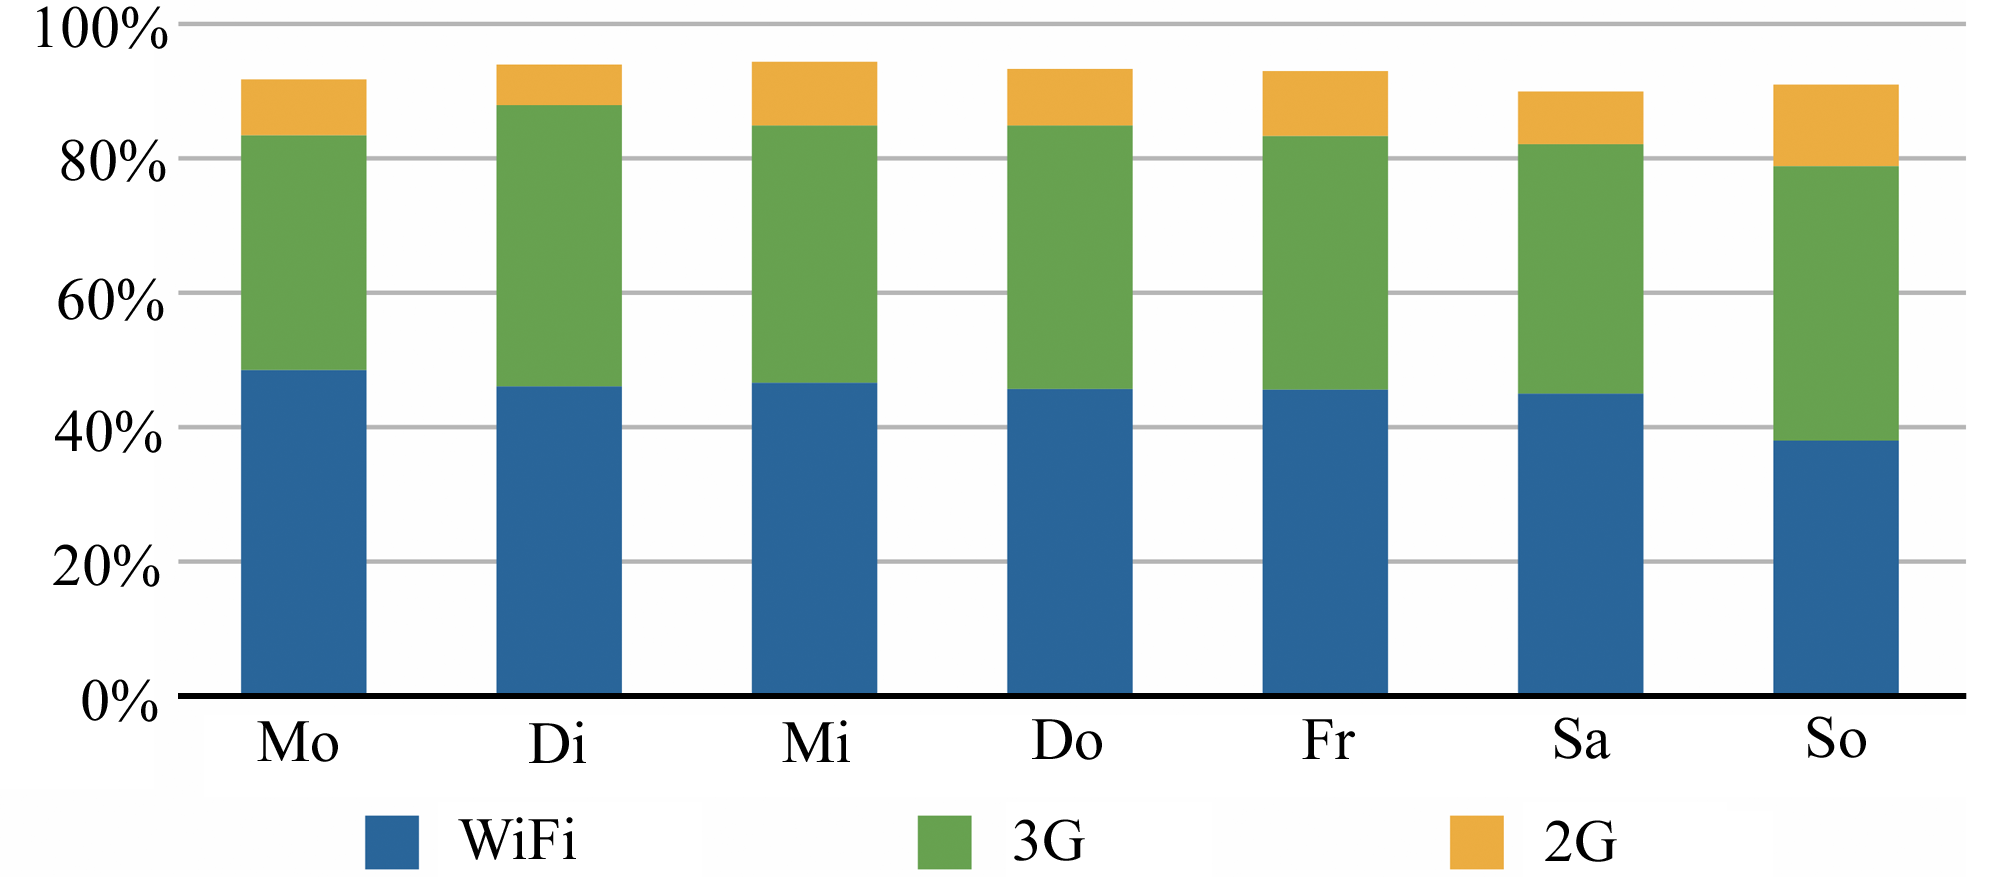
\includegraphics[width=1.0\columnwidth]{images/konnektivitaet}
  \caption{Durchschnittliche tägliche Konnektivität für unterschiedliche Übertragungstechnologien~\protect\cite{o2}} \label{fig:konnektivitaet}
\end{figure}

Unteranderem zeigt die Studie die durchschnittliche tägliche Zeit über einer Woche in Prozent an, in der Benutzer entweder mit 3G/2G oder mit WiFi zum Internet verbunden sind (vgl. Abbildung~\ref{fig:konnektivitaet}).
Es lässt sich feststellen, dass die tägliche Konnektivität über der ganzen Woche mit einer Übertragungstechnologie mit 90\% sehr hoch ist~\cite{o2}.
Die Zeiten der Verbindungsabbrüche lassen sich durch signallose Gebiete (zum Beispiel U-Bahnen) oder durch das Ausschalten des Smartphones erklären~\cite{o2}.
Die Zeiten der Konnektivität der unterschiedlichen Technologien (WiFi, 3G, 2G) über der Woche ist ebenfalls recht stabil.
WiFi erreicht eine durchschnittliche Konnektivität von 45\%, 3G von 40\%~\cite{o2}.
Damit sind Benutzer rund 85\% ihres Tages mit einer Technologie verbunden, die hohe Bandbreiten erlaubt.

Studien~\cite{o8, o12} analysieren die Energieeffizienz durch Computation Offloading anhand der Trade-off-Ungleichung in Kapitel 2 am Beispiel eines Nokia N900.
Dafür vernachlässigen sie die entstehenden Energiekosten des mobilen Geräts beim Warten auf die Beendigung der Berechnung der ausgelagerten Funktion.
Die Studien nehmen für ihre Testzwecke an, dass die entsprechende Cloud-Plattform die Aufgabe schnell lösen kann und das Handy wenig Energie beim Warten verbraucht~\cite{o8}.
Man erhält dadurch eine vereinfachte Trade-Off-Ungleichung~\cite{o8}:

\begin{equation*}
	C\frac{P_{\textit{lokal}}}{X_{\textit{lokal}}} > P_s\frac{D_s}{B_s} + P_e\frac{D_e}{B_e}
\end{equation*}

Nach~\cite{o8} läuft das Nokia N900 mit einer Geschwindigkeit $X_{\textit{lokal}}$ von 600MHz während einer Berechnung und verbraucht dabei 0.9W Leistung pro Sekunde $P_{\textit{lokal}}$.
Studie~\cite{o12} verifiziert diese Ergebnisse.
Damit ergibt sich nach $X_{\textit{lokal}}/P_{\textit{lokal}}$ ungefähr eine Anzahl von 650 Millionen Befehlen pro Joule.
Nach einer Studie der Universität von Helsinki~\cite{o8} sendet und empfängt das Nokia N900 im WiFi bei einer Geschwindigkeit von 700kB/s ungefähr $B_s/P_s = $600kB pro Joule.
Bei einer gedrosselten Verbindung von 100kB/s beträgt die Energieeffizienz 110kB/J.
Ebenso wurde die Energieeffizienz beim Senden und Empfangen im 3G-Netzwerk an unterschiedlichen Standpunkten gemessen (nah und weit entfernt von der Basisstation)~\cite{o12}.
Es zeigt sich, das die Energiekosten zum Übertragen weitaus höher sind als zum Empfangen und die Entfernung zur Basisstation einen signifikanten Unterschied im Bezug auf den Energieverbrauch ausmacht~\cite{o12}.
Unter besten Umständen müssen damit für eine nutzbringende Auslagerung ungefähr eine Millionen Befehle in der Berechnung ausgeführt werden, wenn ein Megabyte an Daten übertragen wird~\cite{o12}.
Dieses Ergebnis deckt sich mit dem Ergebnis aus~\cite{o8}.
Das führt nach~\cite{o8} zu folgenden Entscheidungshilfen:
\begin{enumerate}
	\item Aufgaben mit keiner oder wenig Datenübertragung sollten immer ausgelagert werden
	\item Aufgaben mit komplexen Berechnungen können ausgelagert werden
	\item Aufgaben, die eine größere sekundäre Datenübertragung als die Übertragung zur Auslagerung benötigen, sollten ausgelagert werden
\end{enumerate}

Für das Framework ThinkAir wird ebenso auch eine Evaluierung anhand von mehreren Szenarien unter drei verschiedenen Konnektivitäten (Lokal, WiFi und 3G) präsentiert~\cite{thinkair}.
Das 3G-Netzwerk besitzt dabei eine durchschnittliche RTT von 100ms.
Für das WiFi existieren zwei Testumgebungen, die in der Evaluierung als Durchschnitt berücksichtigt werden: ein WiFi-Router in einer gewöhnlichen Wohnung (RTT 50ms) und ein öffentlicher Wireless Access Point für eine Vielzahl von Benutzern (RTT 200ms)~\cite{thinkair}.
Die Studie testet das Framework dann anhand von vier Applikationsbeispielen, von denen zwei in dieser Arbeit näher vorgestellt werden sollen: eine Gesichtserkennung und ein Virusscanner~\cite{thinkair}.

\subsubsection{Gesichtserkennung}

\begin{figure}
\centering
  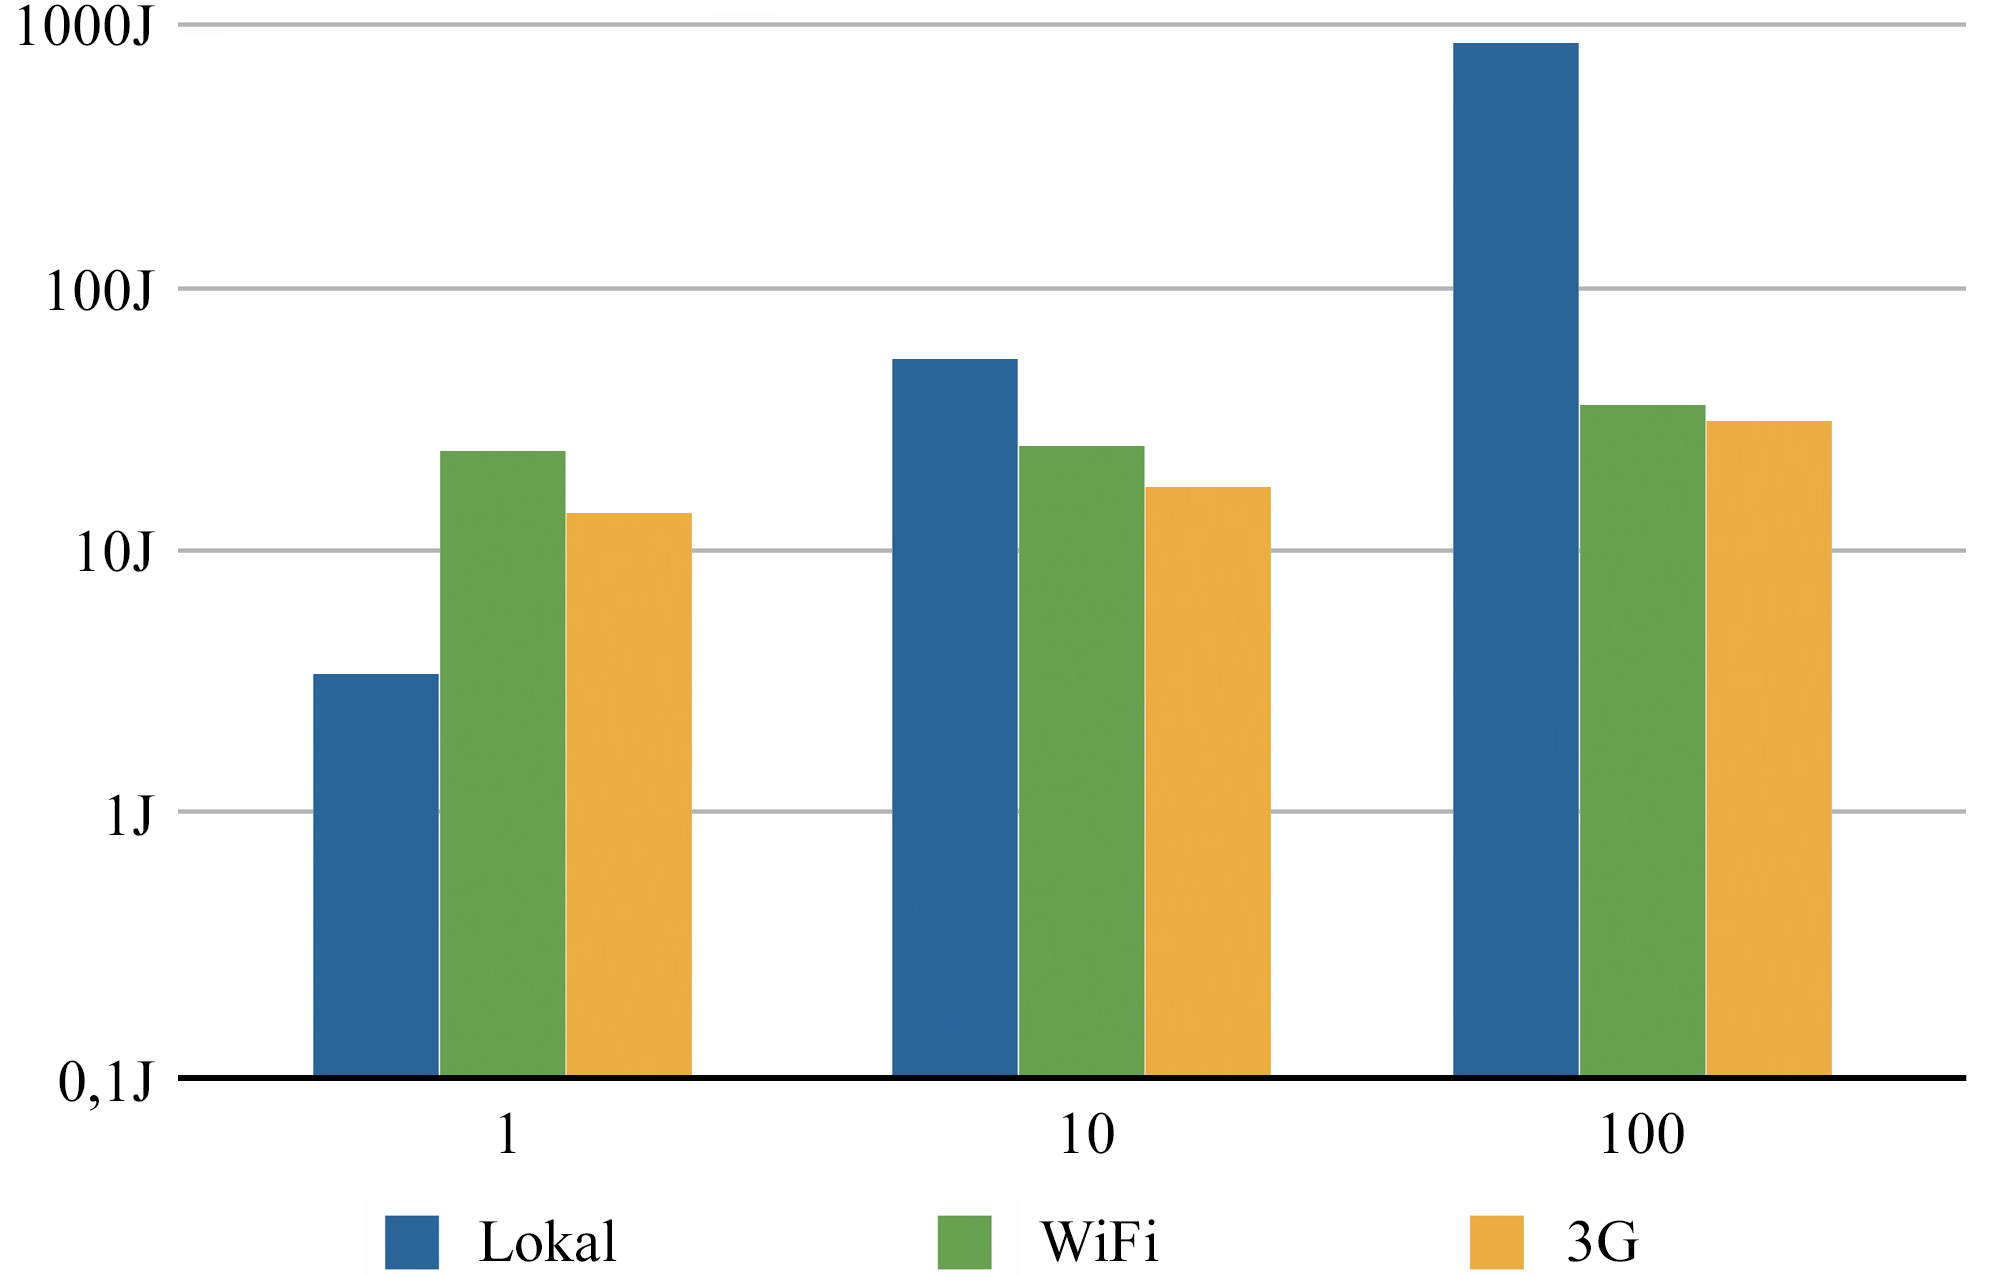
\includegraphics[width=1.0\columnwidth]{images/thinkair}
  \caption{Energieverbrauch bei der Benutzung der unterschiedlichen Über\-tra\-gungs\-tech\-no\-lo\-gien für die Gesichtserkennungs-Applikation nach~\protect\cite{thinkair}}\label{fig:thinkair}
\end{figure}

Die Applikation zählt die Anzahl der Gesichter in einem Bild mit Hilfe der Android API \texttt{FaceDetector}.
Damit ist die Applikation hochgradig für Android optimiert und sollte daher relativ schnell auf dem Smartphone ihre Arbeit verrichten~\cite{thinkair}.
Der Test wird mit einer variablen Anzahl von zu überprüfenden Fotos durchgeführt (1, 10 und 100).
Dabei liegen die Fotos bereits auf dem Smartphone sowie auf der Cloud vor.
Abbildung~\ref{fig:thinkair} präsentiert die Ergebnisse der Gesichtserkennung mit einer logarithmischen Skala.
Die Detektion eines einzelnen Bilds läuft auf dem Smartphone schneller und verbraucht dabei weniger Energie, als wenn die Aufgabe erst über WiFi oder 3G an die Cloud delegiert werden muss.
Steigt die Anzahl der zu analysierenden Fotos, so zeigt sich die Cloud deutlich leistungsstärker und energieeffizienter.
Die Bearbeitung von 100 Fotos verbraucht in der Cloud nur einen Bruchteil der ungefähr 1000J, die lokal zur Berechnung gebraucht würden~\cite{thinkair}.
Der Unterschied zwischen den Übertragungstechnologien WiFi und 3G ist in diesem Beispiel zu vernachlässigen, da keine Daten an die Cloud übertragen werden müssen.

\subsubsection{Virusscanner}
Der Virusscanner ermittelt mittels einer lokalen beziehungsweise in der Cloud liegenden Datenbank mit 1000 enthaltenden Virussignaturen in einem Dateisystem die Anzahl der gefundenen Viren.
Als Testszenario wurden 3500 Daten durchsucht mit einer Gesamtgröße von 10MB~\cite{thinkair}.
Damit müssen im Gegensatz zur Gesichtserkennung in diesem Fall große Datenmengen an die Cloud ausgelagert werden.
Es zeigt sich aber, dass sich die Auslagerung lohnt.
Die Ausführung auf dem Smartphone beträgt für den Scanvorgang über eine Stunde, wohingegen  die Auslagerung und Berechnung in der Cloud nur drei Minuten in Anspruch nimmt.
Die Energieersparnis ist ebenso deutlich.
Verbraucht das Smartphone bei lokaler Berechnung fast 3000 Joule, so werden für die Auslagerung nicht mehr als 70 Joule benötigt~\cite{thinkair}.
Der Unterschied der Energiekosten bei der Übertragung zwischen WiFi und 3G ist erneut marginal.
Es zeigt sich sogar im Gegensatz zu den Studien zum Nokia N900 (vgl.~\cite{o8, o12}), dass die Benutzung von WiFi weniger energieeffizient ist als von 3G~\cite{thinkair}.
Ähnliche Ergebnisse zeigte auch die Gesichtserkennung.

\section{Diskussion}

Wie die Testergebnisse des vorangegangenen Kapitels zeigen, bietet Computation Offloading nicht nur die Möglichkeit der Leistungssteigerung, sondern auch die Einsparung von Energie auf Smartphones bei bestimmten Anwendungsszenarien.
Dabei ist die Einsparung der Energie auch davon abhängig, wie oft das Smartphone mit der Cloud kommuniziert.
Es ist wünschenswert, dass das mobile Gerät jederzeit Daten zur Berechnung an die Cloud senden kann.
Andererseits bremsen langsame oder nicht vorhandene Verbindungen die Akzeptanz und Benutzerfreundlichkeit des Systems.
Wird der Netzwerkprozess eine Qual für den Benutzer, so werden sich diese höchstwahrscheinlich von mobilen Cloud-Systemen abwenden~\cite{o2}.
Computation Offloading-Systeme benötigen sorgsame Planung, um sichtbar lange Latenzzeiten für den Benutzer zu vermeiden~\cite{o12}.
Allerdings schmälern eine durchschnittliche gute Konnektivität von 85\% am Tag und die bereits gute dynamische Entscheidungsfindung der gegenwärtigen Offloading-Frameworks diesen Kritikpunkt~\cite{o2}.
Computation Offloading ist in der heutigen Zeit keine utopische Vorstellung mehr.
Die verbesserte und vermehrte Breitbandabdeckung mit Hilfe von 3G, 4G, Femtozellen und fester Drahtloskommunikation fördern die Bedingungen für Offloading~\cite{thoughtsoncloud}.
Bereits 

Computation Offloading kann weiterhin zum \emph{Mobile Cloud Computing} erweitert werden.
Mobile Cloud Computing bietet zusätzliche Leistungen zum bloßen, effizienteren Berechnen einer Aufgabe.
Zum Beispiel können Benutzerdaten in der Cloud gespeichert werden oder  Inhalte über mehrere Benutzer geteilt werden~\cite{o12}.
Das hat zur Folge, dass für viele Anforderungen die entsprechenden Daten bereits in der Cloud gespeichert sind.
Damit reduziert sich der Netzwerktransfer beim Computation Offloading auf ein Minimum.
Lediglich die Aufforderung zur Berechnung der Aufgabe muss der Cloud mitgeteilt werden~\cite{o12}.
Bereits heute lagern viele Benutzer ihre Daten an die Cloud aus.
Damit wird ihnen eine Sicherheit ihrer Daten garantiert und diese werden verschiedenen Geräten einfach zugänglich gemacht.

Computation Offloading bietet weiterhin den Vorteil, Berechnungen, die sich auf eine Datenbank beziehen, leicht und ohne das Wissen vom Benutzer zu erweitern ohne das dieser durch nervige Updates der Applikation gestört wird.

Auf der anderen Seite ergeben sich neben möglichen langen Latenzzeiten und der dadurch entstehenden Minderung der Benutzerfreundlichkeit noch weitere Nachteile für Benutzer und Entwickler, die unbedingt beachtet werden sollten.

Benutzer von Computation-Offloading-Systemen sollten darüber im Klaren sein, dass ihr Smartphone während der Ausführung der Applikation im ständigen Kontakt zum Internet steht.
Anstehende Traffic-Kosten in Zeiten von Internetflatrates mit Datenlimit können zum Ärgernis des Benutzers führen.
Ebenso ist die Privatsphäre und Sicherheit von sensiblen Daten ein kritischer Punkt bei der Abwägung zum Offloading.
Private Daten werden möglicherweise an Server gesendet, über die der Benutzer keine Kontrolle hat~\cite{o4}.
Der Benutzer sollte entscheiden können, ob er die Auslagerung der Berechnung auf diesen Daten befürwortet oder doch lieber lokal auf dem Smartphone laufen lassen will.
Bei der heutigen Angst der ständigen Überwachung ist auch Sicherheit ein wichtiges Thema~\cite{o4}.
Ein Dritter kann möglicherweise die Daten bei der Übertragung an die Cloud abfangen.
Mit Hilfe von Kryptografie und dem Aufbau von sicheren Verbindungen kann diesem zwar entgegengewirkt werden, es mildert aber eventuell den Gewinn an Energie durch die Auslagerung.
Eine Ansammlung von Studien und Frameworks haben sich in der Vergangenheit bereits dem Thema Sicherheit beim Computation Offloading gewidmet (vgl.~\cite{o4}).

Der Entwickler muss durch die Benutzung von Computation Offloading zusätzliche Kosten aufwenden.
Rein aus energieeffizienten Gründen ist es verständlich, wenn Entwickler auf das Computation Offloading verzichten.
So sollte neben dem Gewinn von Energieeinsparung ebenso der Gewinn an Performance beim Computation Offloading im Vordergrund stehen.
Es scheint schwierig, Entwickler von der Idee des Computation Offloadings zu überzeugen, nur weil Benutzer nicht so gerne ihr Smartphone laden.
Ebenso müssen bei unterschiedlichen App-Versionen möglicherweise verschiedene Smartphone-Klone in der Cloud betrieben werden.

In~\cite{thinkair} wird auch auf mögliche Schwächen im ThinkAir-Framework eingegangen.
So werden bei der Datenübermittlung möglicherweise Instanzobjekte mitgesendet, die für die Berechnung der Methode nicht benutzt werden.
Statische Code-Analysen und das Caching von Objekten in der Cloud sind zwei der vorgeschlagenen Verbesserungsmöglichkeiten~\cite{thinkair}.
So werden Daten, die nicht benutzt werden, und unveränderte Objekte, die bereits in der Cloud liegen, gar nicht erst übermittelt.
Allerdings produziert das Caching von Daten und das Überprüfen auf Veränderungen einen gewissen Mehraufwand, der die Trade-off-Ungleichung verschiebt~\cite{thinkair}.
Daraufhin wird auch auf die Sicherheits-Problematik im ThinkAir-Framework eingegangen.
Ein Vorschlag dafür ist ein Authentifizierungsmechanismus, um eine Verbindung über einen Shared-Secret-Service zu registrieren~\cite{thinkair}.
Für die Übermittlung von privaten Daten, wie dem Standort oder den Profildaten des Benutzers, sollen diese vor Dritten in einer zukünftigen ThinkAir-Version über die \texttt{SecureRemotable}-Klasse abgesichert werden und dem Benutzer damit die Last abnehmen, sich um diese Angelegenheiten zu kümmern~\cite{thinkair}.

\section{Ausblick}

Die \glqq International Data Corporation\grqq\ sagt voraus, dass 70\% der Unternehmen in der Informationstechnikbranche auf eine \glqq Cloud first\grqq-Strategie im Jahr 2016 setzen werden~\cite{thoughtsoncloud}.
Damit rückt auch das Computation Offloading immer mehr in die Köpfe der Entwickler und Anwender.
Fortschritt in der Technologie kann und wird das Computation Offloading nur allgegenwärtiger machen, denn die Trade-off-Beziehung wird damit immer weiter in Richtung Offloading verschoben~\cite{o12}.
Die mobile Breitbandabdeckung zum Beispiel wächst und wird von Jahr zu Jahr schneller~\cite{thoughtsoncloud, thinkair}.
Damit können relativ geringe Round Trip Times und hohe Bandbreiten für die Zukunft prognostiziert werden~\cite{thinkair}.

Dagegen benötigt die Aufrechterhaltung einer konsistenten drahtlosen Verbindungen ohne Verbindungsabbrüche bei sich bewegenden Nutzern weitere Forschung und Entwicklung~\cite{o11}.
Dadurch kann die Ausführungszeit einer Applikation und dessen Energiekosten weiter gespart und die Benutzerfreundlichkeit der App gesteigert werden.
Ein weiteres spannendes Forschungsgebiet ist das Umverteilen von laufenden virtuellen Maschinen ohne Verbindungsabbrüche auf Server, die näher am Benutzer sind, um lange Latenzzeiten zu vermeiden~\cite{o11}.

Ebenso ist das Verlangen nach komplexeren Energie-Profilern auf dem Markt enorm gestiegen~\cite{o12}.
Frameworks wie ThinkAir müssen sich auch heute noch mit Schätzungen vom Energieverbrauch einzelner Methoden zufriedengeben und implizieren somit natürlich eine gewisse Fehlertoleranz bei der Entscheidung zur Auslagerung~\cite{thinkair}.
Ebenso können granularere Energie-Profiler Entwickler zu energieeffizienteren Applikationen motivieren.
Energie-Bugs, welche unerwünschterweise viel Energie verbrauchen, können damit endlich ermittelt werden.

Die zur Verfügung stehenden Ressourcen in der Cloud sind unvorstellbar und bieten Spielraum und Möglichkeiten für gänzlich neue und innovative Applikationen~\cite{o12}.
Smartphone-Apps mit umfangreichen Berechnungen werden dadurch erst wirklich möglich.
So wird zum Beispiel die Datenmenge auf Smartphones auf Grund von einer Anreicherung von Fotos und Videos immer komplexer.
Es reicht nicht mehr aus, diese nur über einen Dateinamen, ein Datum und einen Pfad zu verwalten.
Ebenso wollen Benutzer aber nicht jede einzelne Datei über eine Menge von Schlüsselwörtern näher beschreiben.
Das bietet enormen Raum und Wachstum für Erkennungs- und Datenverwaltungstechnologien, die auf Grund ihrer intensiven Berechnungen nur über Computation Offloading umsetzbar sind~\cite{o12}.
Es wird spannend sein, zu sehen, welche neuen Applikationen über Computation Offloading und der Cloud realisierbar werden~\cite{o12}.

\bibliographystyle{SIGCHI-Reference-Format}
\bibliography{literatur}

\end{document}
